%%
% The BIThesis Template for Bachelor Graduation Thesis
%
% 北京理工大学毕业设计(论文)第一章节 —— 使用 XeLaTeX 编译
%
% Copyright 2020 Spencer Woo
%
% This work may be distributed and/or modified under the
% conditions of the LaTeX Project Public License, either version 1.3
% of this license or (at your option) any later version.
% The latest version of this license is in
%   http://www.latex-project.org/lppl.txt
% and version 1.3 or later is part of all distributions of LaTeX
% version 2005/12/01 or later.
%
% This work has the LPPL maintenance status `maintained'.
%
% The Current Maintainer of this work is Spencer Woo.
%
% 第一章节

\chapter{史瓦西黑洞物理}
\section{黑洞简介}
\subsection{黑洞是什么}
黑洞是一片引力强大到连光都无法逃脱的区域\cite{what_is_black_hole}。银河系的中心就是一个质量为太阳430万倍的黑洞\cite{galactic_center_bh},几乎所有的星系中心都是一个超大质量的黑洞。
\subsection{奇点}
黑洞的中心是一个密度无穷大的奇点,奇点的时空也无限扭曲。黑洞奇点是造成时空扭曲并形成黑洞视界的根源。
\subsection{事件视界}
黑洞的视界是使黑洞称为黑洞的区域,视界以内的信息都无法向外传递,因为没有向外的路径存在。本文研究的限制在视界以外的区域(exterior)。
\subsection{引力透镜}
黑洞(事件视界)根据无毛定理,任何信息都不能从视界上发射出来\footnote{不考虑量子力学},导致黑洞本身是不能被看到的。但黑洞会扭曲周围的时空,通过观察周围物质的运动可以“看”到黑洞。\\
黑洞就像一个圆形或者近似圆形透镜,会使远处传来的平行光产生偏折。

\section{描述弯曲的时空}
\subsection{时间与空间}
狭义相对论开始,时间与空间在洛伦兹变换下被密切的关联起来。从光速不变原理引出长度收缩与时间膨胀的现象。闵可夫斯基时空将时间作为坐标的一个维度,构建了一个四维的坐标系$\left(ct,x,y,z\right)$。刘慈欣在三体中写道,「光锥之内就是命运」\cite{three-body},即是说你所在时空所有光锥之外的事件都与你无关。

\subsection{黎曼几何}
闵可夫斯基时空是一个平直的时空,仅适用于狭义相对论。广义相对论中,时空不再是平直的。要描述一个扭曲的时空,就要用到非欧几何。

\subsection{测地线}
\paragraph{什么是测地线}
测地线是黎曼流形中用于描述两点之间最短路径的曲线,测地线是曲面微分后的最短路径,不是宏观的两点最短路径。测地线是黎曼流形中的直线。测地线应用到非平直时空主要是两种类型。
\paragraph{Timelike 测地线}
光锥之内的测地线称为Timelike 测地线,是有静质量的物体在时空中自由落体所走的路径。
\paragraph{Null 测地线}
当引力场中测试粒子质量降为0时,如光子,在时空运动的轨迹。也就是光锥本身。



\section{史瓦西黑洞性质}
史瓦西度规是一个具有对称性的时空,使用四维球坐标系$\left(ct,r,\theta,\phi\right)$.

史瓦西黑洞具有如下性质:
\begin{enumerate}
    
    \item what
    \item sdfsdf
\end{enumerate}


\section{史瓦西黑洞测地线与光线追踪方程的推导}

史瓦西黑洞测地线
\begin{equation}
    ds^{2}=c^{2}d\tau^{2}=c^{2}\left(1-\frac{2MG}{c^{2}r}\right)dt^{2}-\left(1-\frac{2MG}{c^{2}r}\right)^{-1}dr^{2}-r^{2}d\theta^{2}-r^{2}\sin\theta^{2}d\phi^{2}
\end{equation}
其中$M$是黑洞的质量, $G$是万有引力常数, $c$是真空光速.
对于无质量的粒子(光子)我们有 Null 测地线,
\begin{equation}
    g_{\mu\nu}u^{\mu}u^{\nu}=u^{\mu}u_{\mu}=0
\end{equation}
带入史瓦西黑洞测地线有

\begin{equation}
    \begin{split}
        0 & =-\left(1-\frac{2MG}{c^{2}r}\right)\left(c\frac{dt}{d\tau}\right)^{2}+\left(1-\frac{2MG}{c^{2}r}\right)^{-1}\left(\frac{dr}{d\tau}\right)^{2}\\
        & \qquad+r^{2}\left(\frac{d\theta}{d\tau}\right)^{2}+r^{2}\sin^{2}\theta\left(\frac{d\phi}{d\tau}\right)^{2}
    \end{split}
\end{equation}

因为史瓦西度规是一个球对称时空,粒子的运动可以简化成赤道面上的圆周运动. 令$\theta=\frac{\pi}{2}$, 则$d\theta=0$, 带入得,
\begin{equation}
    \begin{split}
        0&=-\left(1-\frac{2MG}{c^{2}r}\right)\left(c\frac{dt}{d\lambda}\right)^{2}+\left(1-\frac{2MG}{c^{2}r}\right)^{-1}\left(\frac{dr}{d\lambda}\right)^{2}+r^{2}\left(\frac{d\phi}{d\lambda}\right)^{2}
    \end{split}
\end{equation}

根据能量守恒与角动量守恒,我们有两个在时间维度$t$和$\phi$维度的Killing Vector
\begin{equation}
    \begin{split}
        \left(1-\frac{2GM}{c^{2}r}\right)c^{2}\frac{dt}{d\tau}&=\frac{E}{m_{0}}\\
        r^{2}\sin^{2}\theta\frac{d\phi}{d\tau}&=\frac{L}{m_{0}}
    \end{split}
\end{equation}
解得
\begin{equation}
    \begin{split}
        \frac{dt}{d\lambda}&=\left(1-\frac{2GM}{c^{2}r}\right)^{-1}\frac{E}{m_{0}c^{2}}=\left(1-\frac{2GM}{c^{2}r}\right)^{-1}\frac{E}{c^{2}}\\\frac{d\phi}{d\lambda}&=\frac{L}{m_{0}r^{2}\sin^{2}\theta}=\frac{L}{m_{0}r^{2}}=\frac{L}{r^{2}}
    \end{split}
\end{equation}
将其带入,
\begin{equation}
    \begin{split}
        \left(\frac{dr}{d\lambda}\right)^{2}+\frac{L^{2}}{r^{2}}\left(1-\frac{2GM}{c^{2}r}\right)=\frac{E^{2}}{c^{2}}
    \end{split}
\end{equation}
因为角动量$L=\frac{d\phi}{d\lambda}r^{2}$,我们可以消去仿射参数$\lambda$,
\begin{equation}
    \frac{1}{L}\left(\frac{dr}{d\lambda}\right)=\sqrt{\left(\frac{E}{Lc}\right)^{2}-\frac{1}{r^{2}}\left(1-\frac{2GM}{c^{2}r}\right)}
\end{equation}
最终得到一个关于$dr$与$d\phi$的方程,这是最终要在光线追踪过程中要使用的方程
\begin{equation}
    \frac{d\phi}{dr}=\frac{1}{r^{2}\sqrt{\left(\frac{1}{b}\right)^{2}-\frac{1}{r^{2}}\left(1-\frac{2GM}{c^{2}r}\right)}}\label{eq:geodesic}
\end{equation}

\section{光线在史瓦西时空运动规律与程序模拟}
\subsection{Convention}
我们有常量$G$与$c$,设$G=c=1$,则方程的长度单位为黑洞质量$M$,史瓦西半径为$2M$
\subsection{在Mathematica中模拟}
首先设定积分函数

\begin{mma}
    \In |NIntegrate|[|\frac{1}{r^2 \sqrt{\frac{1}{b^2}-\frac{1-\frac{\text{rs}}{r}}{r^2}}}|,\{r, r0, r1\}] \\
\end{mma}
\subsection{撞击参数}
撞击参数$b$有如下定义,
\begin{equation}
    b=\frac{Lc}{E}
\end{equation}
其中$L$是角动量,$c$是真空光速,$E$是粒子的能量。$L$与$E$都是通过守恒原则从Killing Vector中获得的。

从测地线方程中可以看出撞击参数是唯一决定无质量粒子的运动轨迹的参数。我们要获得粒子运动轨迹与粒子发射角度、粒子发射距离的关系,需要重新推导这个关系式。
\begin{equation}
    \begin{split}
        b&=\frac{Lc}{E}\\&=\frac{\vec{r}\times\vec{p}c}{E_{kinetic}+E_{Potential}}\\&=\frac{rp\sin\theta c}{hf+\left(\sqrt{1-\frac{r_{s}}{r}}-1\right)hf}\\&=\frac{rp\sin\theta c}{pc+\left(\sqrt{1-\frac{r_{s}}{r}}-1\right)pc}\\b&=\frac{r\sin\theta}{\sqrt{1-\frac{r_{s}}{r}}}\label{eq:impact_param}
    \end{split}
\end{equation}
其中$\vec{r}$是粒子的方向向量,$\vec{p}$是粒子的动量向量,光子没有静质量,所以我们得到光子的总能量是光子的动量$E_{kinetic}$与光子势能$E_{potential}$。这样我们就得到了发射距离、发射角与撞击参数的关系。

\paragraph{圆周轨道}
从这个关系式\eqref{eq:impact_param}中,令$\theta=\frac{\pi}{2}$可以得到光子的圆周轨道
\begin{equation*}
    \begin{split}
        \frac{b\sqrt{1-\frac{r_{s}}{r}}}{r}&=\sin\theta\\
        b&=\frac{3\sqrt{3}}{2}r_{s}
    \end{split}
\end{equation*}
光子在史瓦西时空只有$r=3M$这一个不稳定轨道。

\paragraph{光子轨道近点}
测地线方程\eqref{eq:geodesic}有奇点,是光子轨道的近点 (Closest Approach),函数在近点不再连续,所以我们需要计算近点$r3$,
\begin{equation}
    b=\frac{r_3}{\sqrt{1-\frac{r_s}{r_3}}}\label{eq:r3}
\end{equation}
这个方程是一个三次方程,需要根据光子的发射距离$r$决定方程的根。

\paragraph{测地线函数图像}
设$r_0$为光子的出发距离,$r_1$为光子的最终距离,$r_3$为光子轨道近点,$\theta$为发射角度。$\text{Position}$轴的前半部分(0-0.5)是光子发射点$r_0$到光子轨道近点$r_3$的线性比例距离,后半部分是近点$r_3$到设定的积分终点$r_1$的线性距离。函数横轴是分两段线性绘制的。图像的不连续点为函数奇点。纵轴Accmulated Phi是积分原点$r_0$到Position $r$的积分,单位为弧度。
\begin{figure}[htbp]
    \centering
    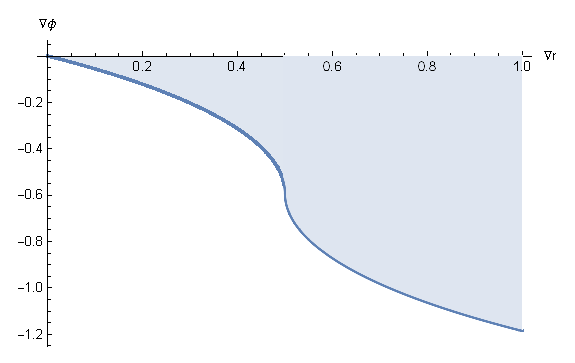
\includegraphics[]{images/dphi_1.eps}
    \caption{$r_0=20M$, $r_1=20M$, $\theta=\frac{\pi}{3}$}\label{dphi_1} % label 用来在文中索引
\end{figure}

\begin{figure}[htbp]
    \centering
    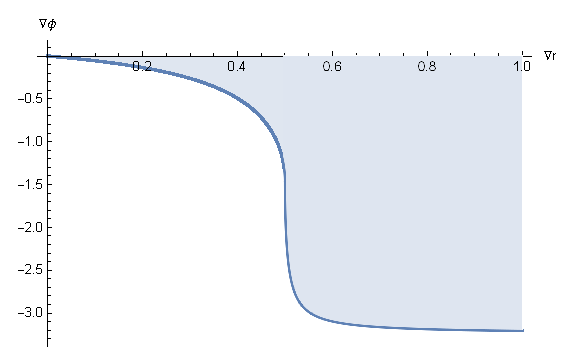
\includegraphics[]{images/dphi_2.eps}
    \caption{$r_0=40M$, $r_1=400M$, $\theta=\frac{\pi}{10}$}\label{dphi_2} % label 用来在文中索引
\end{figure}

\paragraph{赤道面上的光线追踪}
有了$dr$与$d\phi$的关系就可以在赤道面上进行光线追踪了。
